\newpage

\subsection*{Задание 6: Измерение импульсной мощности с помощью осциллографа}
	Для измерения импульсной мощности была собрана следующая схема:\\
	\\
	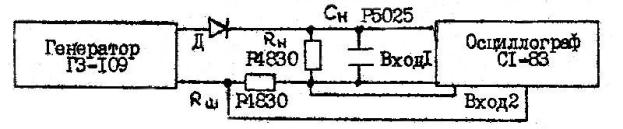
\includegraphics[width=\textwidth]{ch6.jpg}
	\\
	\vspace{1cm}
	\\
	Импульсные сигналы создаются при помощи выпрямления синусоидального напряжения генератора ГЗ-109 посредством диода 
	\textit{Д}. В качестве нагрузки используется параллельное соединение магазинов сопротивления $R_{n}$ типа \textit{P4830} и емкости $C_{n}$ типа \textit{Р5025}. Для регистрации формы тока в нагрузке последовательно с ней включен датчик тока 
	$R_{w}$, напряжение на котором пропорционально току нагрузки. Напряжение с датчика тока и напряжение нагрузки подводится к двухканальному электронному осциллографу типа \textit{C1-83}.
	\vspace{1cm}
	\\
	На выходе генератора \textit{ГЗ-109} устанавливается напряжение 10 \textit{V} и частота 400 \textit{Hz}. Сопротивление нагрузки устанавливается равным $R_{n}$=500 \textit{Ом}, а емкость нагрузки $С_{n}$ =0,5 \textit{мкФ}.
	\vspace{1cm}
	\\
	\textit{\centerline{Графики тока и напряжения с осциллографа:}}
	\\
	\begin{center}
		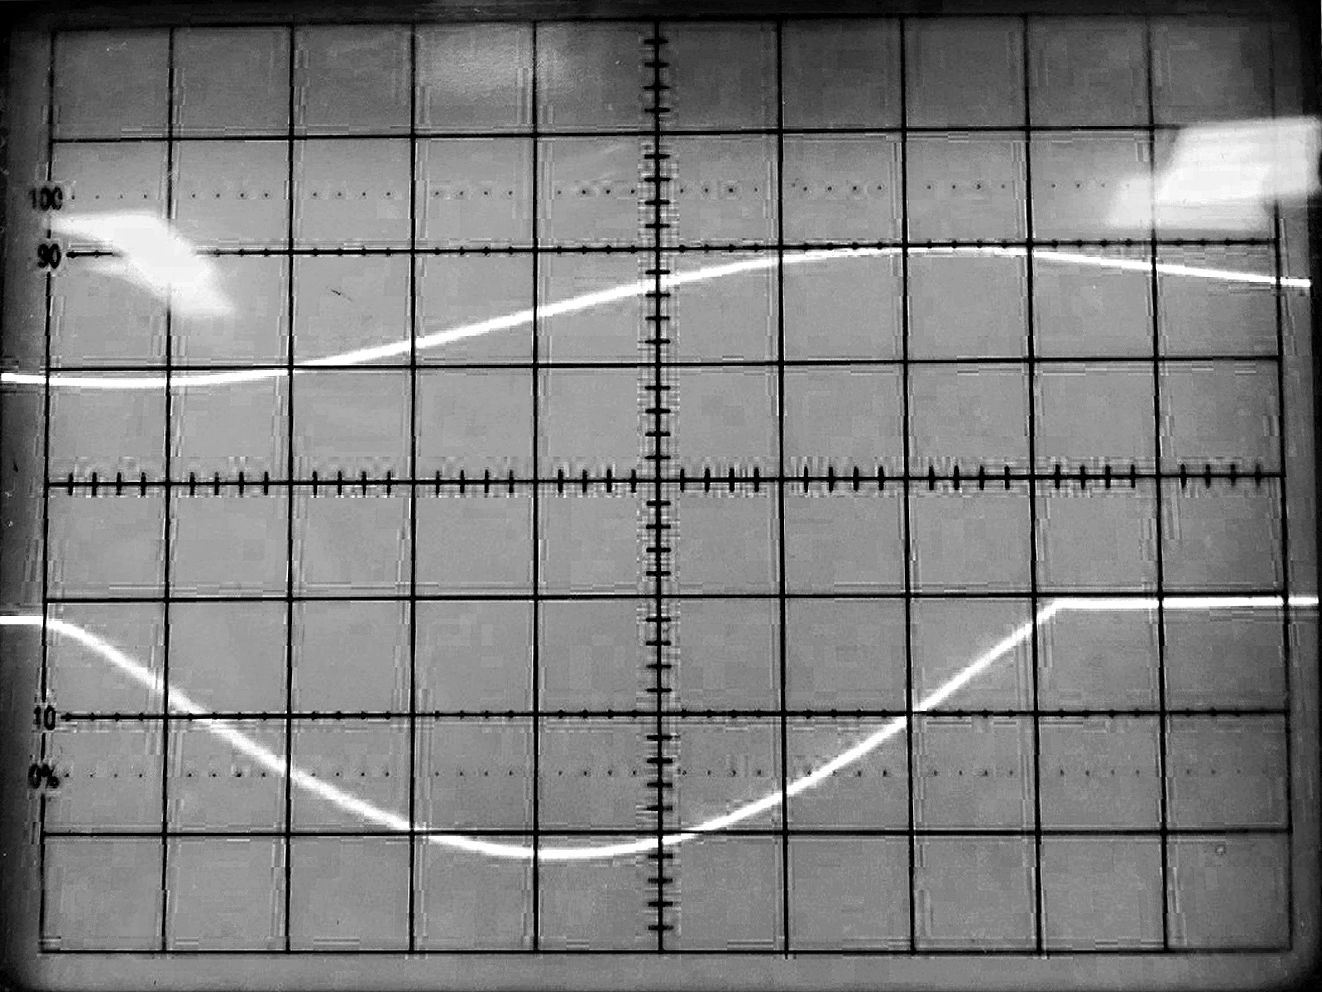
\includegraphics[width=13cm]{graphicVandI.jpg}
	\end{center}


	\newpage
	\textbf{Форма 3} (Результаты измерения напряжения, силы тока и подсчета мгновенной и импульсной мощности):
	\\
	\begin{table}[h!]
		\begin{tabular}{|p{4cm}|p{1.1cm}|p{1.2cm}|p{1cm}|p{1cm}|p{1cm}|p{1cm}|p{1cm}|p{1cm}|p{1.2cm}|}
			\hline
			Номер ординаты $k$: 	   &	 0  &	1	&	2	&	3	&	4	&	5	&	6	&	7	&	8	\\
			\hline
			Напряжение $U_{k}$, ($V$): &	4.5	&	4	&	5	&	6	&	7	&	8.5	&	9	&	10	&	9.5	\\
			\hline
			Ток $I_{k}$, ($A$):		   & 0.015	& 0.04	& 0.075	&  0.1	& 0.11	& 0.105 & 0.09  & 0.05  &	0.01\\
			\hline
			Мощность $P_{k}$, ($W$):   &-0.3825	&-0.29	& -0.075&	0.15&	0.32& 0.4425&	0.36&	0.05&-0.355	\\
			Мощность $P_{u}$, ($W$):   & 0.5284	& 0.5284& 0.5284&0.5284	&0.5284	&0.5284	&0.5284	&0.5284	&0.5284	\\
			\hline
		\end{tabular}
	\end{table}
	\\
	Импульсную мощность выделяют путем графического интегрирования по формуле Симпсона (для \textit{n}=8):\\

	\centerline{$P_{u}$ = $\frac{1}{3n}$ ($P_{k0}$+4($P_{k1}$+$P_{k3}$+$P_{k5}$+$P_{k1}$)+2($P_{k2}$+$P_{k4}$+$P_{k6}$)+$P_{k8}$).}

	\begin{center}
		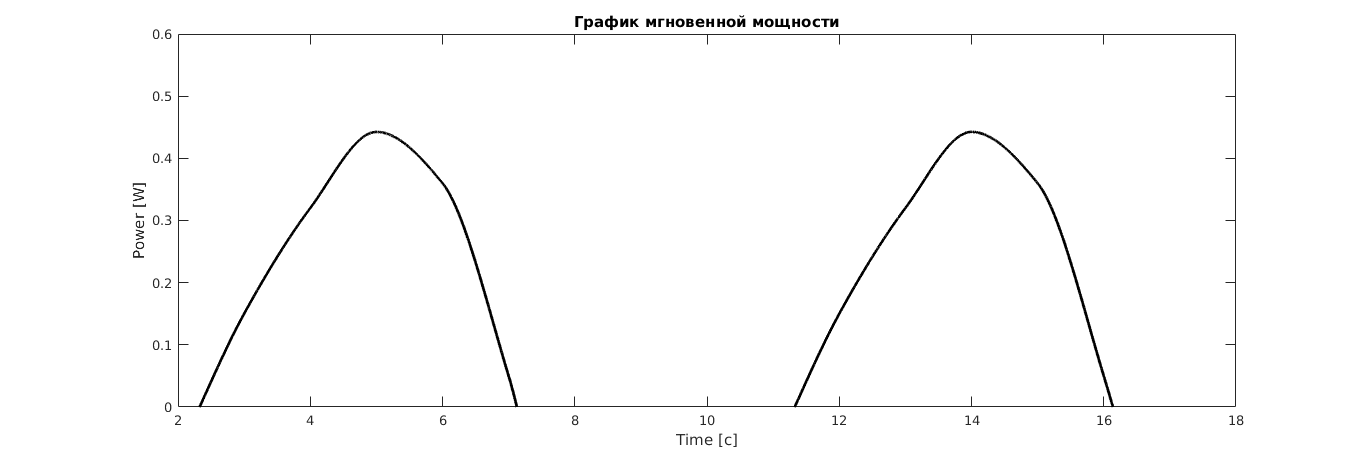
\includegraphics[width=\textwidth]{graphtask2.png}
	\end{center}
